\documentclass[12pt,utf8,notheorems,compress]{beamer}

\usepackage[utf8]{inputenc}
\usepackage[ngerman]{babel}

\usepackage{amsmath,amssymb}
\usepackage{eurosym}
%\usepackage[framed,amsmath,thmmarks,hyperref]{ntheorem}

%\usepackage[small,nohug]{diagrams}
%\diagramstyle[labelstyle=\scriptstyle]

\usepackage[protrusion=true,expansion=false]{microtype}

%\usepackage{lmodern}
\usepackage{tabto}
\usepackage{tikz}
\usepackage{array}
\usepackage[all]{xy}
\usepackage{setspace}
\usepackage{ragged2e}

%\usepackage[natbib=true,style=numeric]{biblatex}
%\usepackage[babel]{csquotes}
%\bibliography{lit}

%\usepackage{hyperref}

\setlength\parskip{\medskipamount}
\setlength\parindent{0pt}

\newcommand{\floatbox}[3]{%
  \raisebox{0pt}[0pt][0pt]{%
    \begin{picture}(0,0)(#1,#2)#3\end{picture}\leavevmode%
  }%
}

\title{Crashkurs Typographie}
\author[Augsburger Off-Topic-Seminar]{Ingo Blechschmidt \\
  Augsburger Off-Topic-Seminar}
\date{??. Juni 2014}

%\usetheme{Warsaw}  %Warsaw, Berkeley?
\usetheme{Warsaw}
\useoutertheme{split}
\usecolortheme{seahorse}
\usefonttheme{serif}
\usepackage{palatino}
\useinnertheme{rectangles}
%\usepackage{bookman}
%\setbeamercovered{transparent}

\setbeamertemplate{navigation symbols}{}
%\setbeamertemplate{footline}{}
\setbeamertemplate{headline}{}

%\beamertemplateboldcenterframetitle
%\setbeamerfont{frametitle}{size={\Large}}

\newcommand*\oldmacro{}%
\let\oldmacro\insertshorttitle%
\renewcommand*\insertshorttitle{%
  \oldmacro\hfill\insertframenumber\,/\,\inserttotalframenumber\hfill}

\newenvironment{changemargin}[2]{%
  \begin{list}{}{%
    \setlength{\topsep}{0pt}%
    \setlength{\leftmargin}{#1}%
    \setlength{\rightmargin}{#2}%
    \setlength{\listparindent}{\parindent}%
    \setlength{\itemindent}{\parindent}%
    \setlength{\parsep}{\parskip}%
  }%
  \item[]}{\end{list}}

\newcommand{\slogan}[1]{%
  \begin{center}%
    \setlength{\fboxrule}{2pt}%
    \setlength{\fboxsep}{-3pt}%
    {\usebeamercolor[fg]{item}\fbox{\usebeamercolor[fg]{normal
    text}\parbox{0.9\textwidth}{\begin{center}#1\end{center}}}}%
  \end{center}%
}

\newcommand{\hil}[1]{{\usebeamercolor[fg]{item}{#1}}}

\newcommand{\img}[2]{\begin{center}\includegraphics[scale=#1]{images/#2}\end{center}}
\newcommand{\imageslide}[2]{\frame{\img{#1}{#2}}}

\newcommand{\nogoslide}[3]{
  \subsection{#1}
  \frame[t]{
    \frametitle{%
      \only<1>{Was ist hier faul?}%
      \only<2->{#1}
    }
    #2
    \vfill
    \only<2->{#3}
  }
}

\newcommand{\nogoslidea}[3]{
  \subsection{#1}
  \frame[t]{
    \frametitle{%
      #1
    }
    #2
    \vfill
    \only<2->{#3}
  }
}

\definecolor{grey}{rgb}{0.3,0.3,0.3}

\begin{document}

\setbeameroption{show notes}
\setbeamertemplate{note page}[plain]

\imageslide{1.1}{sense}

\frame{\titlepage}
%\frame[t]{\frametitle{Gliederung}\begin{minipage}{\textwidth}\begin{small}\tableofcontents\end{small}\end{minipage}}
\setcounter{tocdepth}{1}
\frame[t]{\frametitle{Gliederung}\tableofcontents}

\imageslide{0.4}{serious}

\section{Todsünden}

\nogoslidea{Schriftarten}{
  \only<1>{\img{0.5}{schriftarten}}
  \only<2->{\begin{center}
    \visible<4>{\Huge Serifen \quad \textsf{serifenlos}}
    \vspace{1em}

    \Large
    \only<2>{%
      \begin{minipage}{0.4\textwidth}
        \sffamily
        \raggedright
        \hyphenpenalty=10000
        traditionell seriös \ reif formal \ gelehrt
      \end{minipage}\qquad
      \begin{minipage}{0.41\textwidth}
        \raggedright
        \hyphenpenalty=10000
        glatt \ locker geschmeidig lässig \ zwanglos
      \end{minipage}
    }%
    \only<3->{%
      \begin{minipage}{0.4\textwidth}
        \raggedright
        \hyphenpenalty=10000
        traditionell seriös \ reif formal \ gelehrt
      \end{minipage}\qquad
      \begin{minipage}{0.41\textwidth}
        \raggedright
        \hyphenpenalty=10000
        \sffamily
        glatt \ locker geschmeidig lässig \ zwanglos
      \end{minipage}
    }
  \end{center}}
}{\only<4>{\begin{itemize}
  \item Nicht verschiedene Schriftfamilien mischen!
  \item Auflockerung durch serifenlose Überschriften bei Haupttext mit Serifen
\end{itemize}}}

\nogoslide{Schusterjungen und Hurenkinder}{\img{0.6}{Hurenkind}}{
  \begin{itemize}
    \item Schusterjungen wissen nicht, wohin sie gehen.
    \item Hurenkinder wissen nicht, woher sie kommen.
    \item Allgemeiner: Auf ungünstige Umbrüche achten!
  \end{itemize}
}

\nogoslide{Schlechter Blocksatz}{
  \begin{center}\begin{minipage}{0.7\textwidth}
    \hyphenpenalty=10000
    Lorem ipsum dolor sit amet, consetetur sadipscing elitr, sed diam nonum
    eirmod tempor invidunt ut labore et dolore magna aliquyam erat, sed diam
    voluptua. At vero eos et accusam t justo duo dolores et ea rebum. Stet
    clita gubergren, no sea takimata sanctus est Lorem ipsum dolor sit
    amet.
  \end{minipage}\end{center}
}{\begin{itemize}
  \item Silbentrennung verwenden!
  \item elegant-ly schlecht, ele-gantly okay
\end{itemize}}

\nogoslide{Gießbäche}{
  \begin{center}\begin{minipage}{0.6\textwidth}
    Lorem ipsum dolor sit amet, conseteturi \,sadipscing elitr, sed diam nonumy
    eirmod temporinvi dunt ut labore et dolore magna aliquyam erat, \,sed diam
    voluptua.
  \end{minipage}\end{center}
}{\begin{itemize}
  \item Gießbäche behindern den Lesefluss.
  \item Sätze umformulieren!
  \item Ähnlich: aufeinanderfolgen Zeilen, die mit demselben Buchstaben beginnen
\end{itemize}}

\nogoslide{Zeilenabstand}{
  \only<1>{
    \begin{center}\begin{minipage}{0.7\textwidth}
      \openup -0.3em
      Lorem ipsum dolor sit amet, consetetur sadipscing elitr, sed diam nonumy
      eirmod tempor invidunt ut labore et dolore magna aliquyam erat, sed diam
      voluptua. At vero eos et accusam et justo duo dolores et ea rebum. Stet
      clita kasd gubergren, no sea takimata sanctus est Lorem ipsum dolor sit
      amet.
    \end{minipage}\end{center}
  }
  \only<2>{
    \begin{center}\begin{minipage}{0.7\textwidth}
      \openup 0.3em
      Lorem ipsum dolor sit amet, consetetur sadipscing elitr, sed diam nonumy
      eirmod tempor invidunt ut labore et dolore magna aliquyam erat, sed diam
      voluptua. At vero eos et accusam et justo duo dolores et ea rebum. Stet
      clita kasd gubergren, no sea takimata sanctus est Lorem ipsum dolor sit
      amet.
    \end{minipage}\end{center}
  }
  \only<3>{
    \begin{center}\begin{minipage}{0.7\textwidth}
      \openup 0em
      Lorem ipsum dolor sit amet, consetetur sadipscing elitr, sed diam nonumy
      eirmod tempor invidunt ut labore et dolore magna aliquyam erat, sed diam
      voluptua. At vero eos et accusam et justo duo dolores et ea rebum. Stet
      clita kasd gubergren, no sea takimata sanctus est Lorem ipsum dolor sit
      amet.
    \end{minipage}\end{center}
  }
}{\only<3>{\begin{itemize}
  \item Macht \LaTeX{} von selbst richtig. :-)
\end{itemize}}}
\imageslide{0.5}{heygirl}

\nogoslidea{Bindestriche}{
  \begin{center}\Large
    Augsburg--München

    Englisch--Deutsch

    New York -- Las Vegas -- Phoenix

    15,-- \euro
  \end{center}
}{\begin{itemize}
  \item Viertelgeviertstrich: als Binde- und Trennstrich. -
  \item Halbgeviertstrich: als Gedanken- und Bisstrich. --
  \item Andere Striche werden im Deutschen kaum verwendet.
\end{itemize}}

\nogoslide{Anführungszeichen}{
  \begin{center}\Huge
    "Peter Müller"

    "`Peter Müller"'

    ``Peter Müller''
  \end{center}
}{\begin{itemize}
  \item Im Deutschen: 99unten 66oben
  \item Im Englischen: 66oben 99oben
  \item Know the difference: 20' 50"
\end{itemize}}

\nogoslide{Unterschneidungen (Kerning)}{
  \only<1>{\img{0.7}{kerning}}
  \only<2>{\img{0.7}{VAL_non_kerning}
  \img{0.7}{VAL_kerning}}
}{\begin{itemize}
  \item \TeX macht das meistens von selbst richtig.
  \item Nur sehr selten muss man mit \texttt{\textbackslash!} oder
  \texttt{\textbackslash kern} nachhelfen.
\end{itemize}}
\imageslide{0.5}{pemsbarbershop}

\subsection{Verschiedenes}
\frame[t]{\frametitle{Verschiedenes}
  \begin{itemize}
    \item \textcolor{grey}{Auf guten Kontrast achten.}
    \item \textsc{Kapitälchen} statt GROSSBUCHSTABEN
    \item \oldstylenums{0123456789} statt 0123456789
    \item \ldots statt ... (\texttt{\textbackslash})
    \item Bitte nicht plenken !
    \item Auto\'{}s zu verkaufen!! Für's Leben lernen.
    \item \emph{kursiv} für Betonungen \hfill \textsl{geneigt}
    \item \textbf{fett} für schnelles Suchen
    \item Deutsche bzw. englische Absatzkonvention beachten.
    \item Sätze und Zeilen nicht mit einem Symbol beginnen.
    \item Abgesetzte Formeln in den Textfluss integrieren.
    Nicht mit Doppelpunkten Pausen erzwingen.
    \item Seitenränder nicht zu klein wählen: \\
          45--80 Zeichen pro Zeile sind lesbar.
  \end{itemize}
}

\section{Praktische Tipps}
\frame[t]{\frametitle{Praktische Tipps}
  \begin{itemize}
    \item \LaTeX{} verwenden.
      \only<1>{
        \floatbox{-40}{210}{
\includegraphics[scale=0.5]{images/obvious}}
      }
    \pause
    \item \texttt{\textbackslash documentclass\{scrartcl\}} statt
    \texttt{\textbackslash documentclass\{article\}}
    \item {\scriptsize \texttt{\textbackslash
    usepackage[protrusion=true,expansion=true]\{microtype\}}}
    \item \texttt{%
            \textbackslash{}setlength\textbackslash{}parskip\{\textbackslash{}medskipamount\}
            \textbackslash{}setlength\textbackslash{}parindent\{0pt\}
          }
    \item Tabellen mit \texttt{\textbackslash usepackage\{booktabs\}}
    \item Geschützte Leerzeichen verwenden:
    \texttt{47\~{}Photonentorpedos} \quad
    \texttt{die Funktion\~{}\$f\$}
    \item Dezimalkommata richtig setzen: \texttt{\$3\{,\}141\$}
    \item \LaTeX{} mit \texttt{Tren\textbackslash-nun\textbackslash-gen} helfen.
    \item \texttt{\textbackslash qedhere}
    \item "`pstricks"' (in Anführungszeichen, da man pdflatex verwenden sollte)
  \end{itemize}
}

\frame[t]{%
  \vspace{-3.5cm}%
  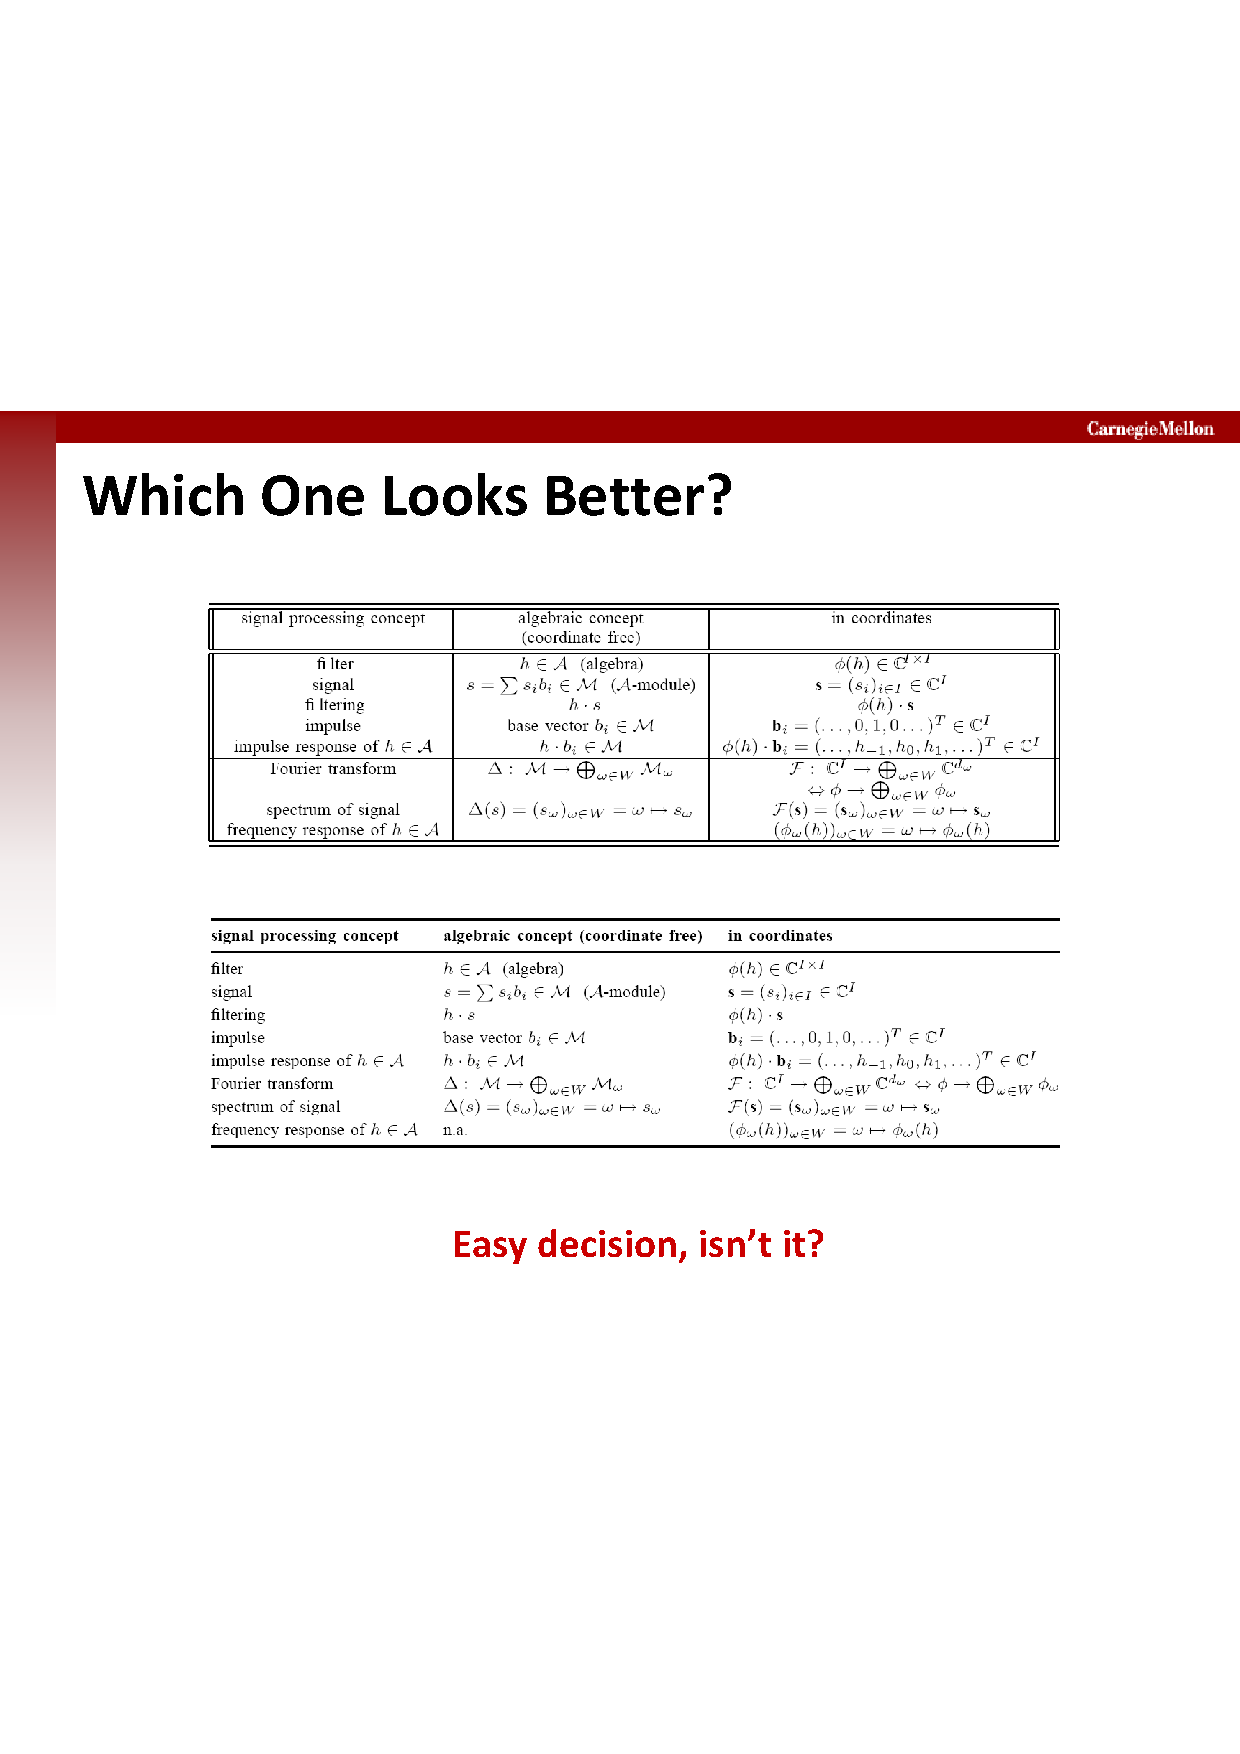
\includegraphics[scale=0.55]{images/tabellen}
}

\section{Endgegner}
\imageslide{0.55}{endgegner}

\frame[t]{\frametitle{Endgegner}
  \justifying
  \small
  Ein \emph{Topos} ist eine Kategorie, die gewisse kategorielle Eigenschaften mit der
  Kategorie der Mengen teilt; das archetypische Beispiel ist die Kategorie der
  Mengen, und das wichtigste Beispiel für die Ziele dieser Notizen ist die
  Kategorie der mengenwertigen Garben auf einem topologischen Raum.

  Jeder Topos~$\mathcal{E}$ unterstützt eine \emph{interne Sprache}. Mit diesem
  Hilfsmittel kann man \emph{vorgeben}, dass die Objekte von~$\mathcal{E}$
  gewöhnliche Mengen und dass die Morphismen gewöhliche Abbildungen zwischen
  diesen Mengen sind -- auch, wenn sie das tatsächlich nicht sind. Sei
  etwa~$\alpha : X \to Y$ ein Morphismus in~$\mathcal{E}$. Von der \emph{internen
  Sicht} sieht dieser wie eine Abbildung zwischen Mengen aus, weswegen wir die
  Bedingung formulieren können, dass diese surjektiv ist; wir schreiben das als
  \[ \mathcal{E} \models \forall y\,{:}\,Y.\ \exists x\,{:}\,X.\ \alpha(x) = y. \]
}

\appendix
\frame[t]{\frametitle{Bildquellen}
  \tiny
  \begin{itemize}
    \item \url{http://ih1.redbubble.net/image.10152097.2266/sticker,375x360.png}
    \item \url{http://img3.wikia.nocookie.net/__cb20070526081820/uncyclopedia/images/1/15/CaptainobviousChooseOption.jpg}
    \item \url{http://imgs.xkcd.com/comics/kerning.png}
    \item \url{http://upload.wikimedia.org/wikipedia/commons/4/44/VAL_kerning.png}
    \item \url{http://upload.wikimedia.org/wikipedia/commons/8/83/VAL_non_kerning.png}
    \item \url{http://wallpepperhd.com/wp-content/uploads/2013/08/Writing-Different-Typography-HD-Wallpaper.png}
    \item \url{http://www.aisleone.net/wp-content/uploads/2009/04/image5.jpg}
    \item \url{http://www.inf.ethz.ch/personal/markusp/teaching/guides/guide-tables.pdf}
    \item \url{http://www.quickmeme.com/img/32/327ecfb57b7090aa945a01870f6fdf36df3bfcb821f81cbd2b70aaaf6ae95476.jpg}
  \end{itemize}
}

\end{document}

